\documentclass{td_um}
\input{../header_td.tex}

\def\version{eno}
%\def\version{cor}

\usepackage{hyperref}
\ue{HAX814X}

\providecommand{\T}{\mathbb{T}}
\providecommand{\1}{\mathds{1}}
\title{TD I}


\newcommand{\miniscule}{\@setfontsize\miniscule{5}{6}}
%-----------------------------------------------------------------------------
\begin{document}
\maketitle

\exo{}
L'étude statistique ci-dessous porte sur les poids (en kg) respectifs des pères $p_{i},$ et ceux de leurs fils aînés $f_{i}$ avec $i=1,\cdots,12$. Les résultats sont tracés sur le graphique suivant

\begin{center}
    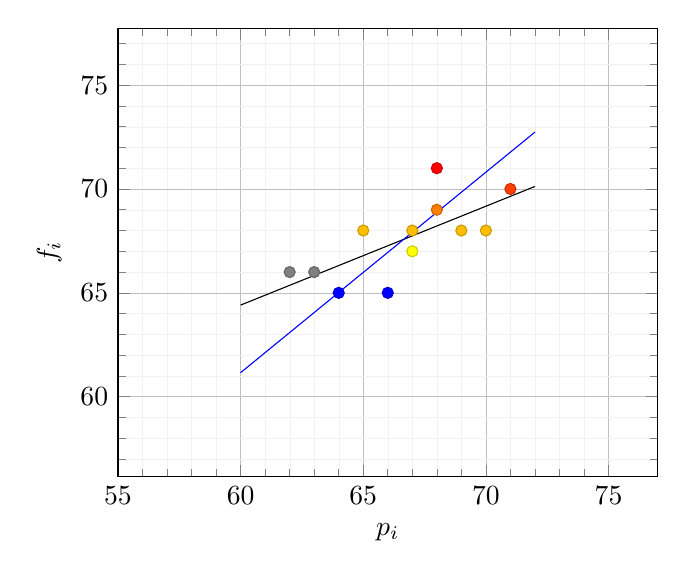
\begin{tikzpicture}
        \begin{axis}[grid=both,%
                grid style={line width=.1pt, draw=gray!10},
    major grid style={line width=.2pt,draw=gray!50},
                minor tick num=4,
                enlargelimits={abs=5},
xlabel=$p_i$,
		ylabel=$f_i$,
            ]
            \addplot[blue,scatter,only marks]%
            table[] {
                x     y  
                65    68 
                63    66 
                67    68 
                64    65 
                68    69 
                62    66 
                70    68 
                66    65 
                68   71  
                67   67  
                69   68  
                71   70  
            };
            \addplot[domain=60:72]{35.85 + 0.476*x};
            \addplot[blue, domain=60:72]{3.258 + 0.965*x};
        \end{axis}
    \end{tikzpicture}
\end{center}

%\[
%\begin{array}{ccccccccccccc}
%p_{i} & 65 & 63 & 67 & 64 & 68 & 62 & 70 & 66 & 68 & 67 & 69 & 71 \\
%f_{i} & 68 & 66 & 68 & 65 & 69 & 66 & 68 & 65 & 71 & 67 & 68 & 70
%\end{array}
%\]
On donne quelques résultats numériques :
$$
\sum p_{i}=800, \sum p_{i}^{2}=53418, \sum p_{i} f_{i}=54107, \sum f_{i}=811, \sum f_{i}^{2}=54849
$$
\begin{enumerate}
    \item  Calculer la droite des moindres carrés du poids des fils en fonction du poids des pères.
    \item  Calculer la droite des moindres carrés du poids des pères en fonction du poids des fils.
    \item  Les deux droites de régression sont-elles identiques?
    \item  En quel point se coupent ces deux droites? Que vaut le produit des pentes des deux droites?
    \item  Estimer $\sigma^{2}$ dans le premier modèle de régression. Un père pèse 70 kilos, peut-il raisonnablement espérer que son fils aîné en pèse $80$?
\end{enumerate}


\cor{\newpage}

\exo{}
Dans de nombreux cas, lorsque l'on étudie le lien entre $Y$ et $X$ nous savons que si $X=0$, alors $Y=0$. On peut alors simplifier le modèle linéaire en cherchant juste à ajuster les points sur une droite d'ordonnée à l'origine nulle. On étudie la régression linéaire $y_{i}=\beta x_{i}+\varepsilon_{i},$ où les $\varepsilon_{i}$ sont centrées, non corrélées et de même variance $\sigma^{2}$. On considère les deux estimateurs de $\beta$ suivants
\[
\hat{\beta}=\frac{\sum_{i=1}^{n} x_{i} y_{i}}{\sum_{i=1}^{n} x_{i}^{2}} \quad \text { et } \quad \tilde{\beta}=\frac{\sum_{i=1}^{n} y_{i}}{\sum_{i=1}^{n} x_{i}}
\]
\begin{enumerate}
    \item  Quelle est la logique de construction de ces deux estimateurs?
    \item   Montrer que $\hat{\beta}$ et $\tilde{\beta}$ sont des estimateurs non biaisés de $\beta$.
    \item   Montrer que la variance de $\tilde{\beta}$ est strictement plus grande que la variance de
        $\hat{\beta},$ sauf dans le cas où les $x_{i}$ sont tous égaux. Ce résultat était-il prévisible?
\end{enumerate}


\cor{\newpage}

\exo{}
On suppose que le modèle de régression linéaire simple de $Y$ en fonction de $X$, avec des erreurs centrées et non corrélées, est valide:
\[
Y=\beta_{0}+\beta_{1} X+\varepsilon
\]
Montrer qu'alors il en est de même pour le modèle de régression linéaire de $X$ en fonction de $Y$. Quels sont les paramètres de ce modèle?


\cor{\newpage}

\exo{}
On considère un objet dont le coût de fabrication est $x_{0}$. Supposons que le nombre d'objets vendus en une semaine, $y$ dépend du prix de vente $x$ selon un modèle linéaire simple.
\begin{enumerate}
    \item  Quel est le prix de vente maximisant la marge de l'entreprise?
    \item  Sur les trois dernières semaines, un industriel a vendu objet
    \[
            \begin{array}[]{cccc}
                \hline
                \text{prix} & 113 & 115 & 120 \\
                \text{quantité} & 230 & 200 & 125 \\
                \hline
            \end{array}
        \]
        Sachant que le coût de fabrication est de $100$ euros, quel prix de vente lui conseillez-vous?
\end{enumerate}


\cor{\newpage}

\exo{} 
Soit $y_{1}, \cdots, y_{n}$ des réels. Pour mesurer l'écart d'un réel $x$ à l'ensemble des $y_{i},$ on peut utiliser la distance $D(x)=\sum_{i=1}^{n} f\left(y_{i}-x\right)$ où $f$ est une fonction positive, paire, s'annulant en 0, contiue et croissante sur les réels positifs.
\begin{enumerate}
    \item Montrer que le réel qui minimise cette distance lorsque $f(t)=t^{2}$ est la moyenne des $y_{i}$
    \item On suppose maintenant que $f(t)=\abs{t}$. Montrer que le réel qui minimise la distance $D(x)$ est la médiane des $y_{i}$. {\it Indication: on considérera que $y_{1} \leq$ $\cdots \leq y_{n}$ et on réécrira $D(x)$ sur l'intervalle $[y_{j}, y_{j+1}[$. On traitera ensuite cas où $n=2 p+1,$ puis le cas où $n=2 p$}.

\end{enumerate}

\cor{\newpage}

\exo{} Soit $y_{1}, \cdots, y_{n}$ et $x_{1}, \cdots, x_{n}$ des réels. Dans le modèle linéaire simple $y_{i}=\beta_{0}+\beta_{1} x_{i}+\varepsilon_{i}$, on considère la somme des erreurs en valeur absolue
\[
    S\left(\beta_{1}, \beta_{2}\right)=\sum_{i=1}^{n}\abs{y_{i}-\beta_{0}-\beta_{1} x_{i}}
\]
et on notera $\tilde{\beta}_{0}$ et $\tilde{\beta}_{1}$ les estimateurs des moindres valeurs absolues, \textit{i.e.} les valeurs de $\beta_{0}$ et $\beta_{1}$ minimisant la fonction $S(\cdot, \cdot)$. On cherche une stratégie pour obtenir $\tilde{\beta}_{0}$ et $\tilde{\beta}_{1}$.
\begin{enumerate}
 \item La valeur de $\beta_{1}$ étant fixée, quelle est la valeur de $\beta_{0}$ qui minimise la fonction $g\left(\beta_{0}\right)=\sum_{i=1}^{n}\left|y_{i}-\beta_{0}-\beta_{1} x_{i}\right| ?$
 \item En déduire un algorithme pour obtenir $\tilde{\beta}_{0}$ et $\tilde{\beta}_{1}$.
\end{enumerate}


\cor{\newpage}

\exo{}
Montrer que le coefficient de détermination $R^{2}$ est égal au carré du coefficient de corrélation empirique entre les $x_{i}$ et les $y_{i}$ défini par
\[
\rho(x, y)=\frac{s_{x y}}{s_{x} s_{y}}=\frac{\sum_{i=1}^{n}\left(x_{i}-\bar{x}\right)\left(y_{i}-\bar{y}\right)}{\sqrt{\sum_{i=1}^{n}\left(x_{i}-\bar{x}\right)^{2} \sum_{i=1}^{n}\left(y_{i}-\bar{y}\right)^{2}}}
\]

\cor{\newpage}


\exo{}
Dans le modèle linéaire simple, si on considère la normalité des $\varepsilon_{i},$ on sait que $y_{i} \sim \mathcal{N}\left(\beta_{0}+\beta_{1} x_{i}, \sigma^{2}\right), \forall i=1, \cdots, n$
\begin{enumerate}
    \item  Exprimer la vraisemblance des observations $L\left(\beta_{0}, \beta_{1}, \sigma^{2}\right)$.
    \item  Quelles sont les valeurs de $\beta_{0}$ et $\beta_{1}$ maximisant cette vraisemblance?
    \item  Quelle est la valeur de $\sigma^{2}$ maximisant cette vraisemblance? Que peut-on alors dire de l'estimateur du maximum de vraisemblance (EMV) de $\sigma^{2}$ ?
\end{enumerate}

\cor{\newpage}

\exo{Intervalles de confiance vs Région de confiance} On considère le modèle de régression linéaire simple $y=\beta_{0}+\beta_{1} x+\varepsilon$. Soit un échantillon $(x_{i}, y_{i})_{i=1}^{100}$ de statistiques résumées
$$
\sum_{i=1}^{100} x_{i}=0 \quad \sum_{i=1}^{100} x_{i}^{2}=400 \quad \sum_{i=1}^{100} x_{i} y_{i}=100 \quad \sum_{i=1}^{100} y_{i}=100 \quad \hat{\sigma}^{2}=1 .
$$
\begin{enumerate}
    \item  Exprimer les intervalles de confiance à $95 \%$ pour $\hat\beta_{0}$ et $\hat\beta_{1}$.
    \item  Donner l'équation de la région de confiance à $95 \%$ de $\hat\beta = \left(\hat\beta_{0}, \hat\beta_{1}\right) .$ \textit{Rappel : l'ensemble des points $(x, y)$ tels que $\frac{\left(x-x_{0}\right)^{2}}{a^{2}}+\frac{\left(y-y_{0}\right)^{2}}{b^{2}} \leq 1$ est l'intérieur d'une ellipse centrée en $(x_{0}, y_{0})$ dont les axes sont parallèles à ceux des abscisses et des ordonnées, et de sommets $(x_{0} \pm a, 0)$ et  $(0, y_{0} \pm b)$.}
    \item  Représenter sur un même graphique les résultats obtenus.
    \end{enumerate}

\end{document}

